\documentclass[a4paper,11pt]{article}

\usepackage[left=2cm, top=3cm, text={17cm, 24cm}]{geometry}
\usepackage[czech]{babel}
\usepackage[utf8]{inputenc}
\usepackage{times}
\usepackage[unicode]{hyperref}
\usepackage{amsmath}
\usepackage{graphicx}
\usepackage{float}
\usepackage[margin=0.5cm]{caption}
\graphicspath{ {./img/} }
\hypersetup{hypertexnames = false}

\begin{document}
	\begin{titlepage}
		\begin{center}
			\textsc{\Huge Vysoké učení technické v~Brně\\
				\vspace{0.4em}\huge Fakulta informačních technologií}
			
			\vspace{\stretch{0.382}}
			
			{\LARGE Modelování a simulace\\
				\Huge Predikce epidemie COVID-19\\ \vspace{0.3em}}
			
			\vspace{\stretch{0.618}}
			
			{\Large \hfill Radek Švec (xsvecr01)\\ \today \hfill Martin Kostelník (xkoste12)}
		\end{center}
	\end{titlepage}

	\section{Úvod}
		Tématem práce jsou epidemiologické modely na makroúrovni, konkrétně předpověď šíření pandemie COVID-19 na území Itálie a České republiky. Tato práce implementuje již existující model, který předpovídá vývoj pandemie na území Itálie, a opakuje provedené experimenty. Tento model byl vytvořen Guiliou Giordanem a dalšími \cite{source}. Smyslem projektu je předpovědězení šíření nemoci COVID-19 na území České republiky v následujících měsících, aplikování různých opatření proti šíření a zhodnocení, zda byly dosavadně zavedené opatření dostačující, případně zda bylo rozvolnění těcho opatření správným rozhodnutím.
		
	\subsection{Autoři a zdroje informací}
		Autory tohoto projektu jsou:
		\begin{itemize}
			\item Radek Švec, xsvecr01@stud.fit.vutbr.cz
			\item Martin Kostelník, xkoste12@stud.fit.vutbr.cz
		\end{itemize}
	
	Jak bylo řečeno v úvodu, samotný model byl převzat z odborné literatury \cite{source}. Při pokusu aplikovat model na prostředí České republiky byly použity data z oficiálních stránek ministerstva zdravotnictví České republiky \cite{mzcr}.
	
	\subsection{Ověření validity}
		Validitu modelu jsme ověřovali zkoumáním převzatého modelu, zejména porovnání výsledků prováděných simulací s reálným vývojem pandemie v Itálii. Validita modelu v prostředí České republiky je opět ověřována porovnáním simulačních dat s reálnými.
	
	\section{Rozbor tématu a použitých metod/technologií}
		
	
	\subsection{Popis použitých postupů}
		Model byl převzat z odborného článku \cite{source} publikovaného v časopise Nature Medicine\footnote{https://www.nature.com/nm/}. Bylo tedy nutné model detailně nastudovat a zkontrolovat dosažené výsledky. Tento konkrétní model nám přišel na modelování pandemie vhodný, jelikož rozděluje společnost do většího množství skupin a počítá s různě těžkými projevy nemoci.
	
	\subsection{Popis použitých technologií}
		Pro provedení experimentů bylo nutné vytvořit simulační model, který jsme implementovali v jazyce C++. Nebylo třeba použít nestandardní knihovny, jelikož se model skládá pouze z řady diferenciálních rovnic. Pro generování grafů byl použit nástroj GNUPlot\footnote{http://www.gnuplot.info/}.
	
	\pagebreak		
	\section{Koncepce abstraktího modelu}
		Model zvaný SIDARTHE je rozšířením jednoduššího SIR modelu, který rozděluje populaci na tři skupiny lidí (náchylní, infikovaní a vyléčení) o dalších pět skupin. Vzniká nám tedy následujících osm skupin.
		
		\begin{itemize}
			\item S -- Náchylní (Susceptible) k onemocnění.
			\item I -- Nakažení (Infected) - asymptomatičtí, vir u nich nebyl detekován.
			\item D -- Diagnostikovaní (Diagnosed) - asymptomatičtí, vir u nich byl detekován.
			\item A -- Nemocní (Ailing) - symptomatičtí, nebyli testováni.
			\item R -- Léčící se (Recognized) - symptomatičtí, byl u nich detekován vir.
			\item T -- Životně ohrožení (Threatened) - mají těžký průběh nemoci, vyžadují intenzivní péči.
			\item H -- Vyléčení (Healed).
			\item E -- Mrtví (Extinct).
		\end{itemize}
	
		\begin{figure}[H]
			\caption{Grafické znázornění modelu, převzato z \cite{source} a přeloženo}
			\label{fig1}
			\centering
			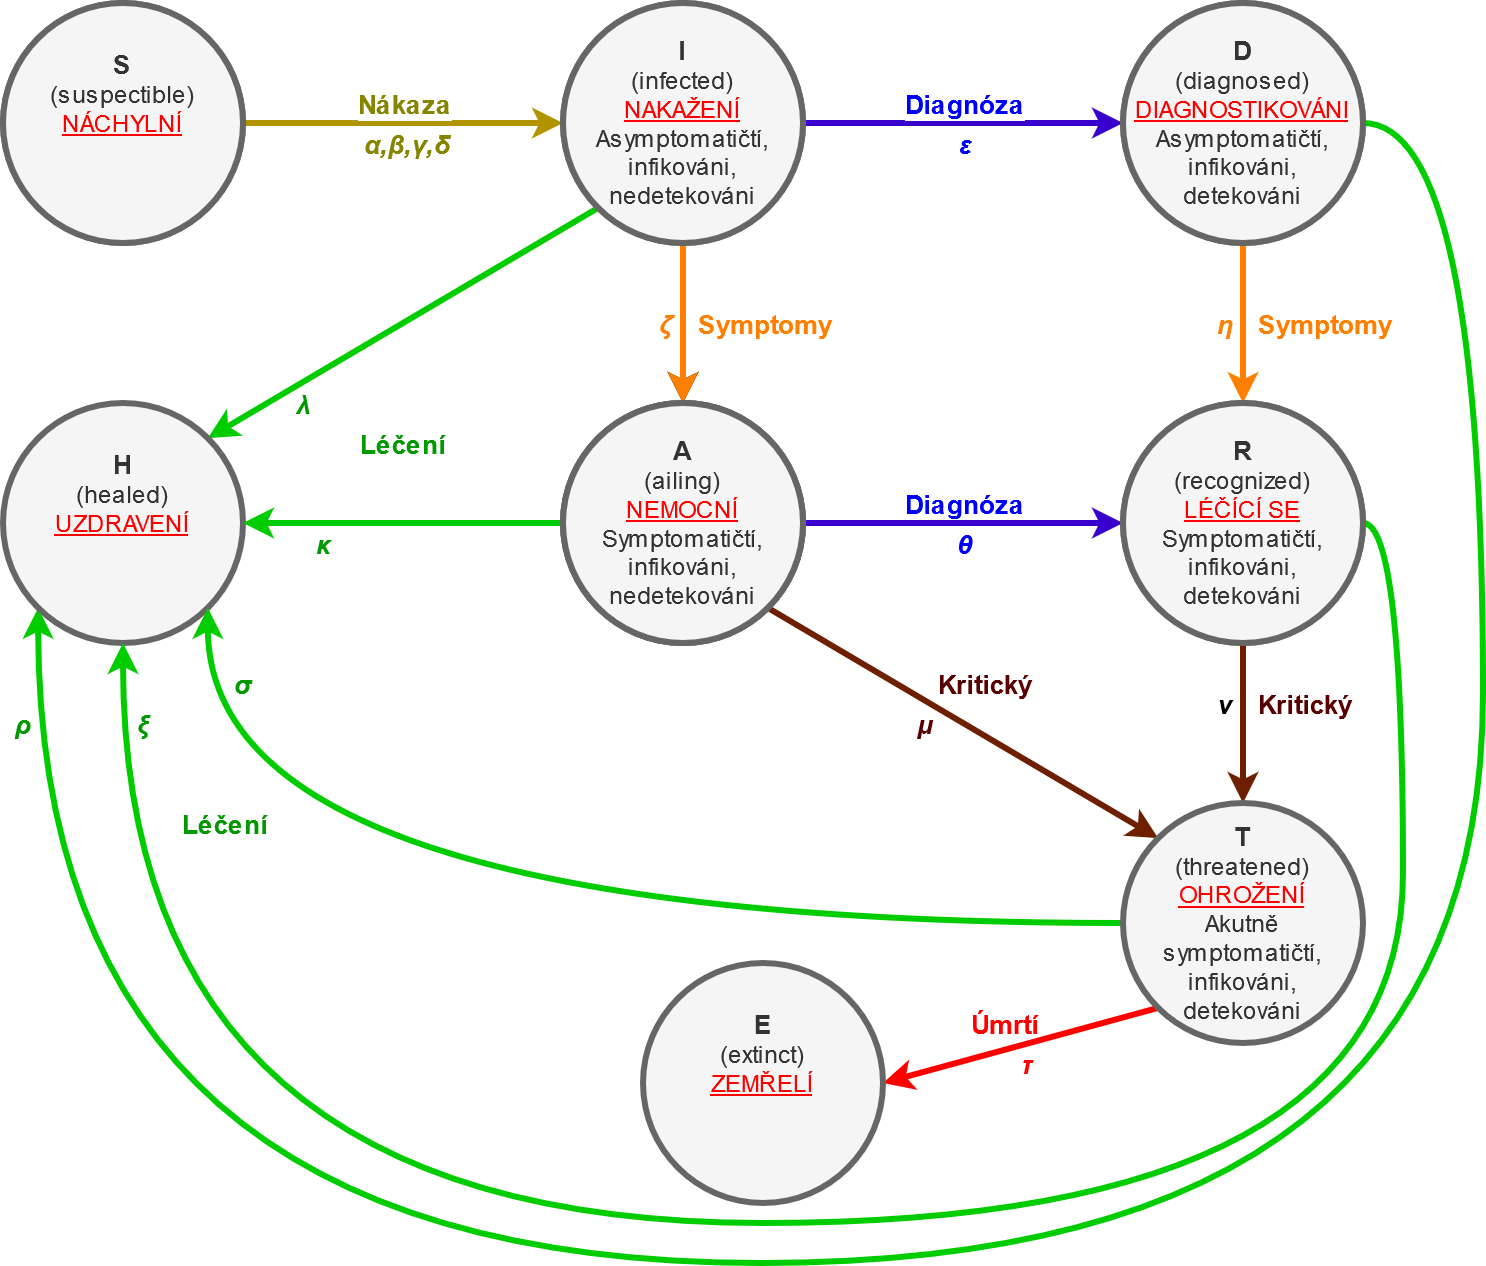
\includegraphics[scale=0.25]{model.png}
		\end{figure}
	
		Tento model nepočítá s možností, že se jedinec může virem nakazit opakovaně. I když bylo prokázáno, že se jedinec znovu nakazit může \cite{reinfection}, není stále přesně známo, jakou imunitu si jedinec vybuduje. Takto nakažených je navíc velice malé množštví, například ve Švédsku v polovině října to bylo pouhých 150 případů \cite{reincases}, tudíž je v modelu zanedbáváme.
		
		\subsection{Matematické vyjádření modelu}
		\label{mathmodel}
		Model můžeme matematicky popsat celkem osmi diferenciálními rovnicemi, které popisují vývoj jedinců v každé skupině jako zlomek celkové populace státu v čase $t$.
		
		\begin{align}
			S'(t) &= - S(t) (\alpha I(t) + \beta D(t) + \gamma A(t) + \delta R(t))\\
			I'(t) &= S(t) (\alpha I(t) + \beta D(t) + \gamma A(t) + \delta R(t)) - (\epsilon + \zeta + \lambda)I(t)\\
			D'(t) &= \epsilon I(t) - (\eta + \rho) D(t)\\
			A'(t) &= \zeta I(t) - (\theta + \mu + \kappa) A(t)\\
			R'(t) &= \eta D(t) + \theta A(t) - (\nu + \xi) R(t)\\
			T'(t) &= \mu A(t) + \nu R(t) - (\sigma + \tau) T(t)\\
			H'(t) &= \lambda I(t) + \rho D(t) + \kappa A(t) + \xi R(t) + \sigma T(t)\\
			E'(t) &= \tau T(t)
		\end{align}
	
	Kromě množství jedinců ve skupinách, se v rovnicích vyskytují následující paramtry:
	\begin{itemize}
		\item $\alpha$, $\beta$, $\gamma$, $\delta$ -- pravděpodobnost přenosu viru mezi náchylným, infikovaným, diagnostikovaným, nemocným a léčícím se jedincem, vynásobenou průměrným počtem kontaktů za den.
		\item $\epsilon$, $\theta$ -- pravděpodobnost detekce viru u nakažených a nemocných.
		\item $\zeta$, $\eta$ -- pravděpodobnost, že se u nakaženého a diagnostikovaného jedince vystkytnou symptomy nemoci.
		\item $\mu$, $\nu$ -- pravděpodobnost, že se z nemocného a léčícího se jedince stane kriticky ohrožený jedinec.
		\item $\tau$ -- úmrtnost.
		\item $\lambda$, $\kappa$, $\xi$, $\rho$ a $\sigma$ -- pravděpodobnost, že se nakažený, nemocný, léčící se, diagnostikovaný, nebo ohrožený jedinec z nemoci vyléčí.
	\end{itemize}
		
	\section{Architektura simulačního modelu}
		V implementovaném programu existují dvě struktury, kde jsou uložena všechna data pro provádění simulací. První struktura v sobě uchovává počty jedinců ve skupinách a další informace o území, na kterém se experimenty provádí. V této struktuře je také implementováno chování modelu, které za pomocí druhé struktury a aktuálních informací předpovídá vývoj nemoci. To se provádí iterováním výpočtů. Druhá struktura popisuje aktuální chování nemoci -- obsahuje všechny paramtery pravděpodobnostního charakteru, jež se využívají v simulacích pro určité časové období a pomáhají k lepší definici následků zpřísnění nebo rozvolnění opatření.
		
		U tohoto modelu je problematické zadání všech parametrů uživatelem. Uživatel by musel zadat velké množství hodnot a tento přístup by byl velice náchylný k chybám. Proto jsou údaje pro všechny provedené experimenty uloženy přímo ve zdrojovém kódu programu. Jednotlivé experimenty je možné spouštět různými cíly definovanými v souboru \texttt{Makefile}. Konkrétní příkazy pro spuštění experimentů jsou v kapitole \ref{experiments}.
		
		Po provedení simulace program vypíše výsledné množství jedinců v každé ze skupin na standardní výstup a zároveň data z každého dne zapisuje do souboru \texttt{data.txt} pro možnost generování grafů.
		
		\subsection{Mapování abstraktního modelu do modelu simulačního}
			Diferenciální rovnice popsané v kapitole \ref{mathmodel} jsou implementovány ve funkci \texttt{predict()}, která je uložena ve struktuře s názvem \texttt{SIDARTHE}. Tato funkce bere na vstupu tři parametry. Prvním je struktura \texttt{Disease} popisující nemoc, druhým a třetím parametrem je počáteční a koncový den simulace. Funkce poté iterativně počítá přírustky jedinců do každé ze skupin a každá iterace představuje jeden den.
			
	\section{Podstata simulačních experimentů a jejich průběh}
	\label{experiments}
		Experimentování s modelem je rozděleno do dvou částí. V první části se pokusíme zopakovat některé experimenty prováděny autory modelu \cite{source}. Ve druhé části aplikujeme model na prostředí České republiky, kde budeme zkoumat vývoj pandemie v období od 1. listopadu 2020 do 31. ledna 2021 a pokusíme se zhodnotit zavedené opatření a případně doporučit zavedení dalších opatření v blízké době.
		
	\section{Zopakování experimentů}
		V této kapitole se pokusíme zopakovat některé z již provedených experimentů a porovnat naše výsledky s referenčními.
	
		\subsection{Experiment 1}
		\label{e1}
			Experiment lze replikovat spuštěním příkazu \texttt{make run1}.
		
			Tento experiment se snaží simulovat šíření nemoci v Itálii od 20. února 2020 do 5. dubna 2020. Celkem se tedy zkoumá čtyřicet šest dní. Během této doby byla v Itálii implementována řada opatření, jejichž následky můžeme sledovat v obrázku \ref{fig2}.
			
			Výstup programu:
			
			TODO: VYSTUP PROGRAMU PRO EXPERIMENT 1

			
			\begin{figure}[H]
				\caption{Porovnání výsledků}
				\label{fig2}
				\centering
				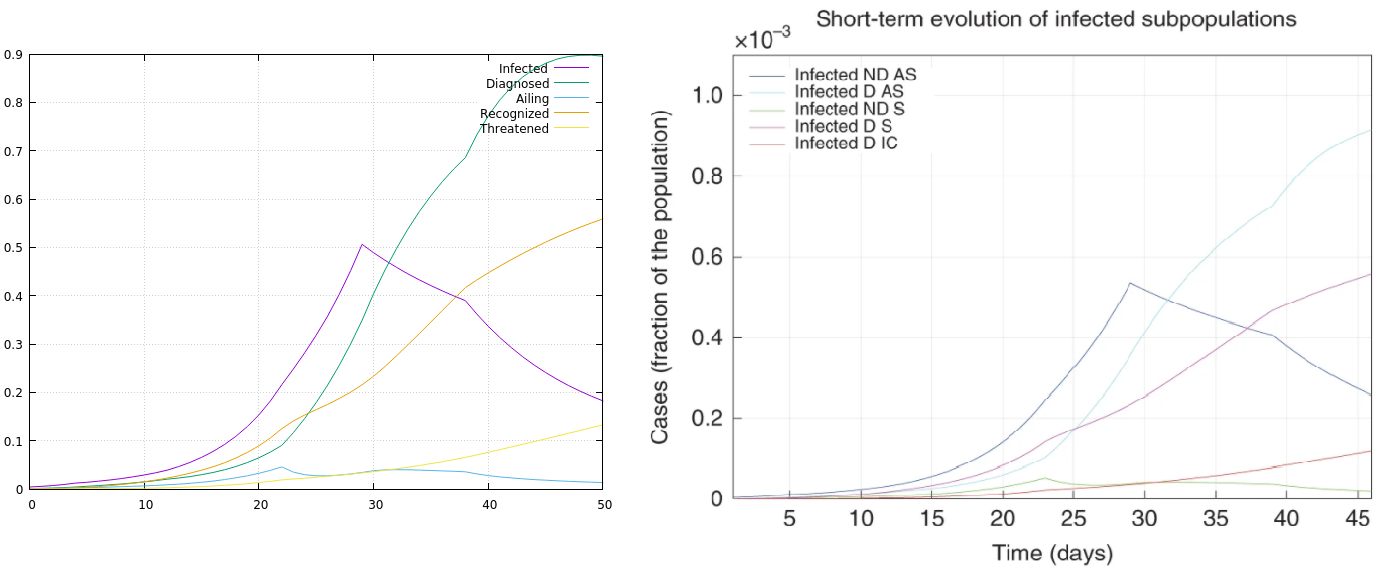
\includegraphics[scale=0.6]{comparison.png}
			\end{figure}
			
			Na levém obrázku můžeme vidět graf generovaný z výsledků našeho experimentu. Na pravém obrázku je graf referenční (převzat z \cite{source}). 
			
		\subsection{Experiment 2}
			Tento experiment navazuje na experiment \ref{e1}. Pokouší se simulovat šíření nemoci na větším časovém úseku. 
		
	\section{Aplikování modelu na Českou republiku}
	
	\section{Shrnutí simulačních experimentů a závěr}
		asdfasdfasdfasdfasdfasdfasdfasdfasdfasdfasdfasdfasdf
		asdfasdfasdfasdfasdfasdfasdfasdf

	\newpage
	\bibliographystyle{czechiso}
	\renewcommand{\refname}{Literatura}
	\bibliography{doc}
\end{document}